\videotitle{Success Stories}

%----------------------------------------------------------------------
\begin{frame}[c]{Spearmint \litw{\href{https://papers.nips.cc/paper/4522-practical-bayesian-optimization-of-machine-learning-algorithms.pdf}{Snoek et al. 2012}}}

\small
\begin{itemize}
    \item First successful open source Bayesian optimization implementation     
%    \item Was used to tune a neural network to state-of-the-art performance on CIFAR-10 in 2012
    \item Implements standard Bayesian optimization with MCMC integration of the acquisition function, asynchronous parallelism, 
    input warping 
    and constraints
    \item \alert{Startup based on Spearmint got acquired by Twitter in 2015}
    \item Still heavily used and cited and available at \url{https://github.com/HIPS/spearmint}:
    \begin{center}
        \only{
\includegraphics[width=0.7\linewidth, keepaspectratio=true]{images/success_stories/jsnoek_spearmint_git_stats.png}}
        
        \only{
\includegraphics[width=0.7\linewidth, keepaspectratio=true]{images/success_stories/hips_spearmint_git_stats.png}}
        
        \only{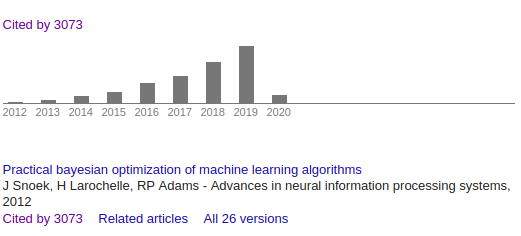
\includegraphics[width=.5\linewidth, keepaspectratio=true]{images/success_stories/spearmint_alt_stats.png}}
%        \newline Google Scholar screenshot from 3rd March, 2020
    \end{center}
\end{itemize}
\end{frame}

%-----------------------------------------------------------------------
\begin{frame}[c]{Hyperopt \litw{\href{https://papers.nips.cc/paper/4443-algorithms-for-hyper-parameter-optimization.pdf}{Bergstra et al. 2011}, \href{http://proceedings.mlr.press/v28/bergstra13.pdf}{Bergstra et al., 2013}, \href{http://citeseerx.ist.psu.edu/viewdoc/download?doi=10.1.1.704.3494&rep=rep1&type=pdf}{Bergstra et al., 2013}, \href{https://iopscience.iop.org/article/10.1088/1749-4699/8/1/014008/ampdf}{Bergstra et al., 2015}}}
\begin{itemize}
    \item Hyperopt is another successful open source Bayesian optimization package
    \item Implements the TPE algorithm and supports asynchronous parallel evaluations
    \item Maintained since 2013
    \item Available at \url{https://github.com/hyperopt/hyperopt}
\end{itemize}
\vspace{1cm}

\includegraphics[width=\linewidth, height=\textheight, keepaspectratio=true]{images/success_stories/hyperopt_git_stats.png}

\vspace{1cm}
\hspace{2cm}


\end{frame}

%---------------------------------------------------------------------
\begin{frame}[c]{SMAC  \litw{\href{https://ml.informatik.uni-freiburg.de/papers/11-LION5-SMAC.pdf}{Hutter et al. 2011}}}

\begin{itemize}
    \item Standard BO tool based on random forests (RFs), reflecting the strengths of RFs in terms of \alert{scalability \& flexibility}:
    \begin{itemize}
        \item High dimensionality (low effective dimensionality)
        \item Computational efficiency ($\rightarrow$ low overhead)
        \item Supports continuous/categorical/conditional parameters
        \item Supports non-standard noise (non-Gaussian, heteroscedastic)
        \item Usability off the shelf (robustness towards model's own hyperparameters)
    \end{itemize}

\fhpause
\smallskip
    \item SMAC also handles a more general problem:
    $\argmin_{\conf\in\confs} \sum_{i=1}^N \cost(\conf,i)$
\fhpause
\smallskip
    \item Maintained since 2011, now available in version 3: \url{https://github.com/automl/SMAC3}

\begin{columns}
\column{0.05\textwidth}
\column{0.45\textwidth}
~\\
%\vspace*{0.1cm}
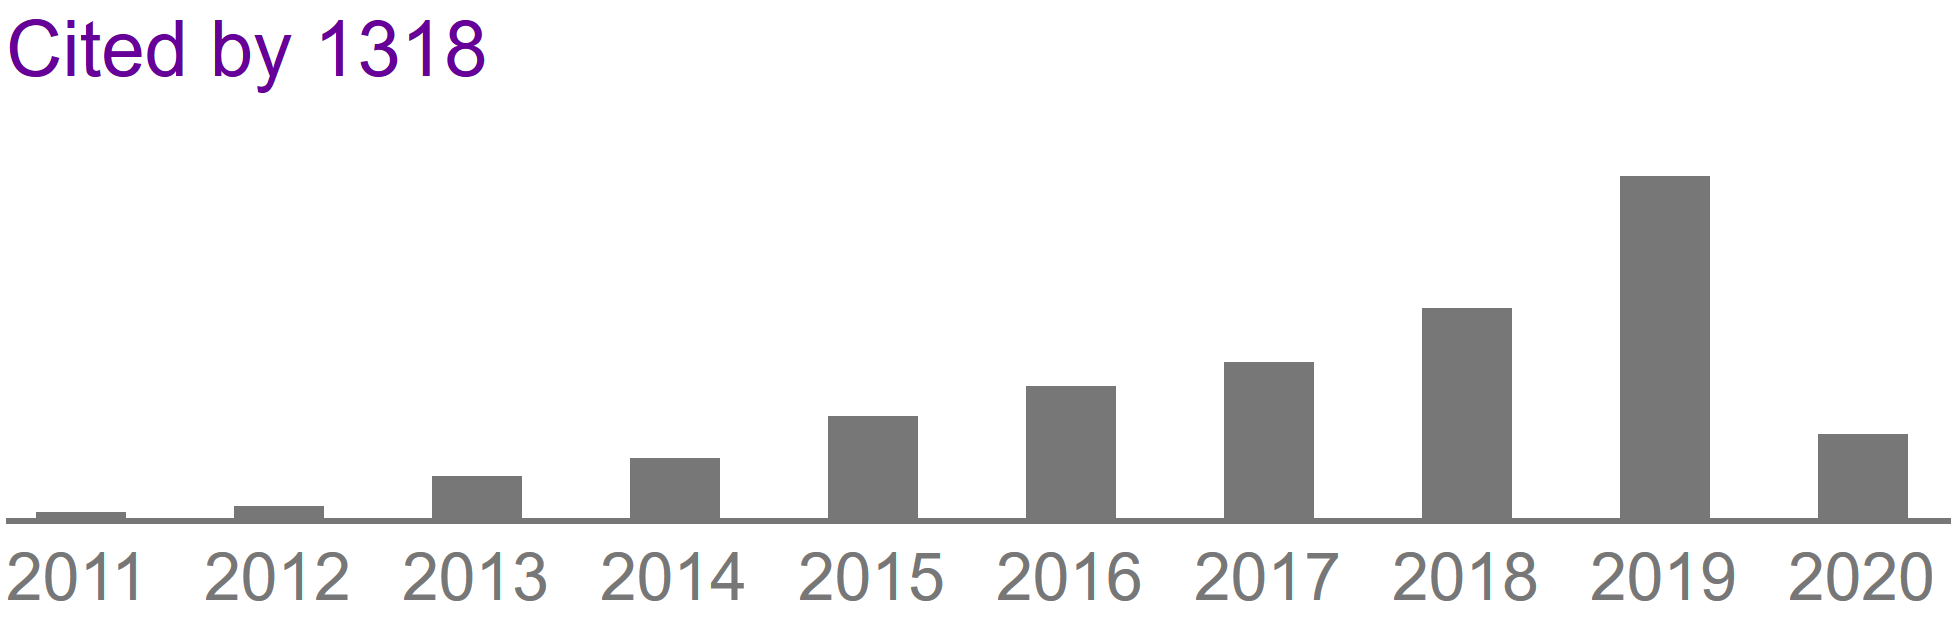
\includegraphics[width=1\linewidth, keepaspectratio=true]{images/success_stories/SMAC_citations.png}
\column{0.45\textwidth}
~\\
~\\
~\\
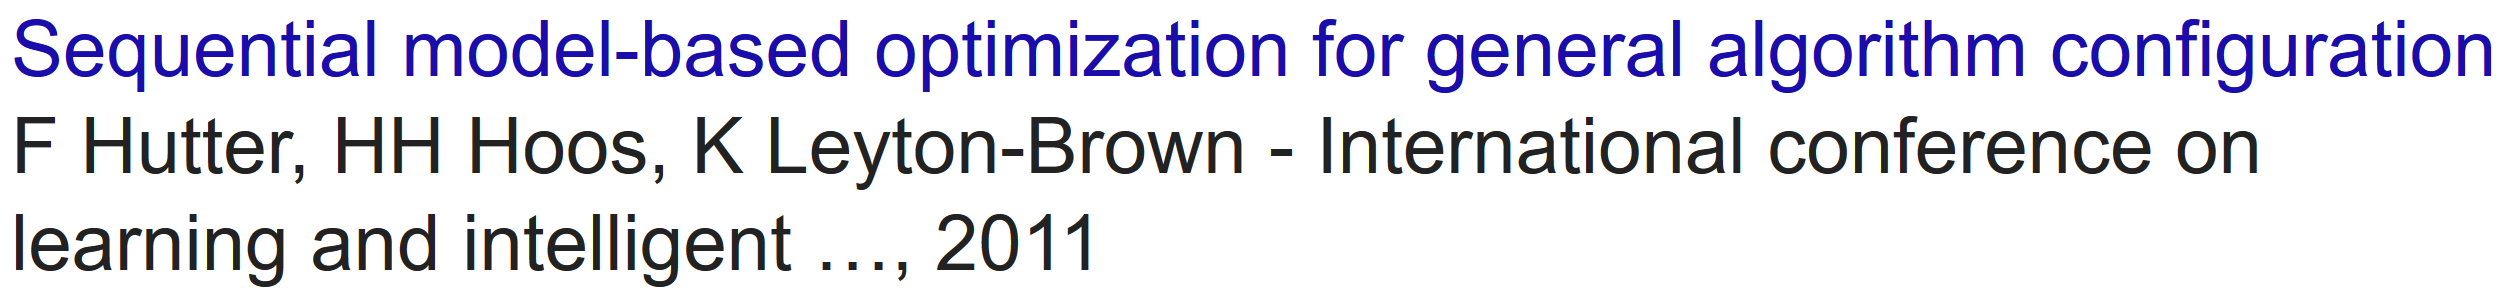
\includegraphics[width=1\linewidth, keepaspectratio=true]{images/success_stories/SMAC_paper.png}
~\\
\column{0.05\textwidth}
\end{columns}    
\end{itemize}
\end{frame}
%----------------------------------------------------------------------

%-----------------------------------------------------------------------
\begin{frame}[c]{Tuning AlphaGo \litw{\href{https://arxiv.org/abs/1812.06855}{Chen et al. 2018}}}
\begin{itemize}
    \item ``During the development of AlphaGo, \alert{its many hyperparameters were tuned with Bayesian optimization multiple times.}''
\medskip
    \item ``This automatic tuning process resulted in \alert{substantial improvements in playing strength}. For example, prior to the match with Lee Sedol, we tuned the latest AlphaGo agent and this \alert{improved its win-rate from 50\% to 66.5\%} in self-play games. \alert{This tuned version was deployed in the final match.}
\medskip
    \item Of course, since we tuned AlphaGo many times during its development cycle, the \alert{compounded contribution was even higher than this percentage.}
\end{itemize}

\end{frame}

%-----------------------------------------------------------------------
\begin{frame}[c]{Company usage}
\begin{itemize}
    \item SIGOPT: startup offering Bayesian optimization as a service
    \item Facebook provides an open source Bayesian optimization package \lit{\href{https://botorch.org/}{BoTorch}}
    \item Amazon provides an open source Bayesian optimization package \lit{\href{https://amzn.github.io/emukit/}{EmuKit}}
    \item Uber tunes algorithms for \emph{Uber Pool}, \emph{UberX} and \emph{Uber Eats} \lit{\href{http://mcqmc2016.stanford.edu/Frazier-Peter.pdf}{source}}
    \item Many more, but less openly
\end{itemize}
\end{frame}

%-----------------------------------------------------------------------
\begin{frame}[c]{Auto-WEKA \litw{\href{https://dl.acm.org/doi/10.1145/2487575.2487629}{Thornton et al, 2013}, \href{http://www.jmlr.org/papers/volume18/16-261/16-261.pdf}{Kotthoff et al, 2017}, \href{https://link.springer.com/chapter/10.1007/978-3-030-05318-5_4}{Kotthoff et al. 2019}}}

    \myit{
        \item First \alert{general AutoML system}, carrying out  \alert{\textbf{C}ombined \textbf{A}lgorithm \textbf{S}election and \textbf{H}yperparameter optimization} (CASH), jointly optimizing
        \begin{itemize}
            \item Choice of algorithm (out of 26 classifiers)
            \item The algorithm's hyperparameters (up to 10)
            \item Choice of preprocessing method and its hyperparameters
            \item Choice of ensemble \& meta methods
        \end{itemize}
    }

\begin{columns}
\column{0.0\textwidth}
\column{0.55\textwidth}

\onslide<2->
\vspace*{-0.4cm}
    \myit{
        \item Parameterized WEKA \lit{\href{https://www.cs.waikato.ac.nz/ml/weka/Witten_et_al_2016_appendix.pdf}{Frank et al, 2016}}: \alert{768 hyperparameters}, 4 leves of conditionality
    }
    \onslide<3->{
    \myit{\item Optimized 10-fold cross-validation via SMAC 
    \lit{\href{https://ml.informatik.uni-freiburg.de/papers/11-LION5-SMAC.pdf}{Hutter et al, 2011}}
    }
    }
\column{0.45\textwidth}
\vspace*{-0.4cm}
\onslide<2->{
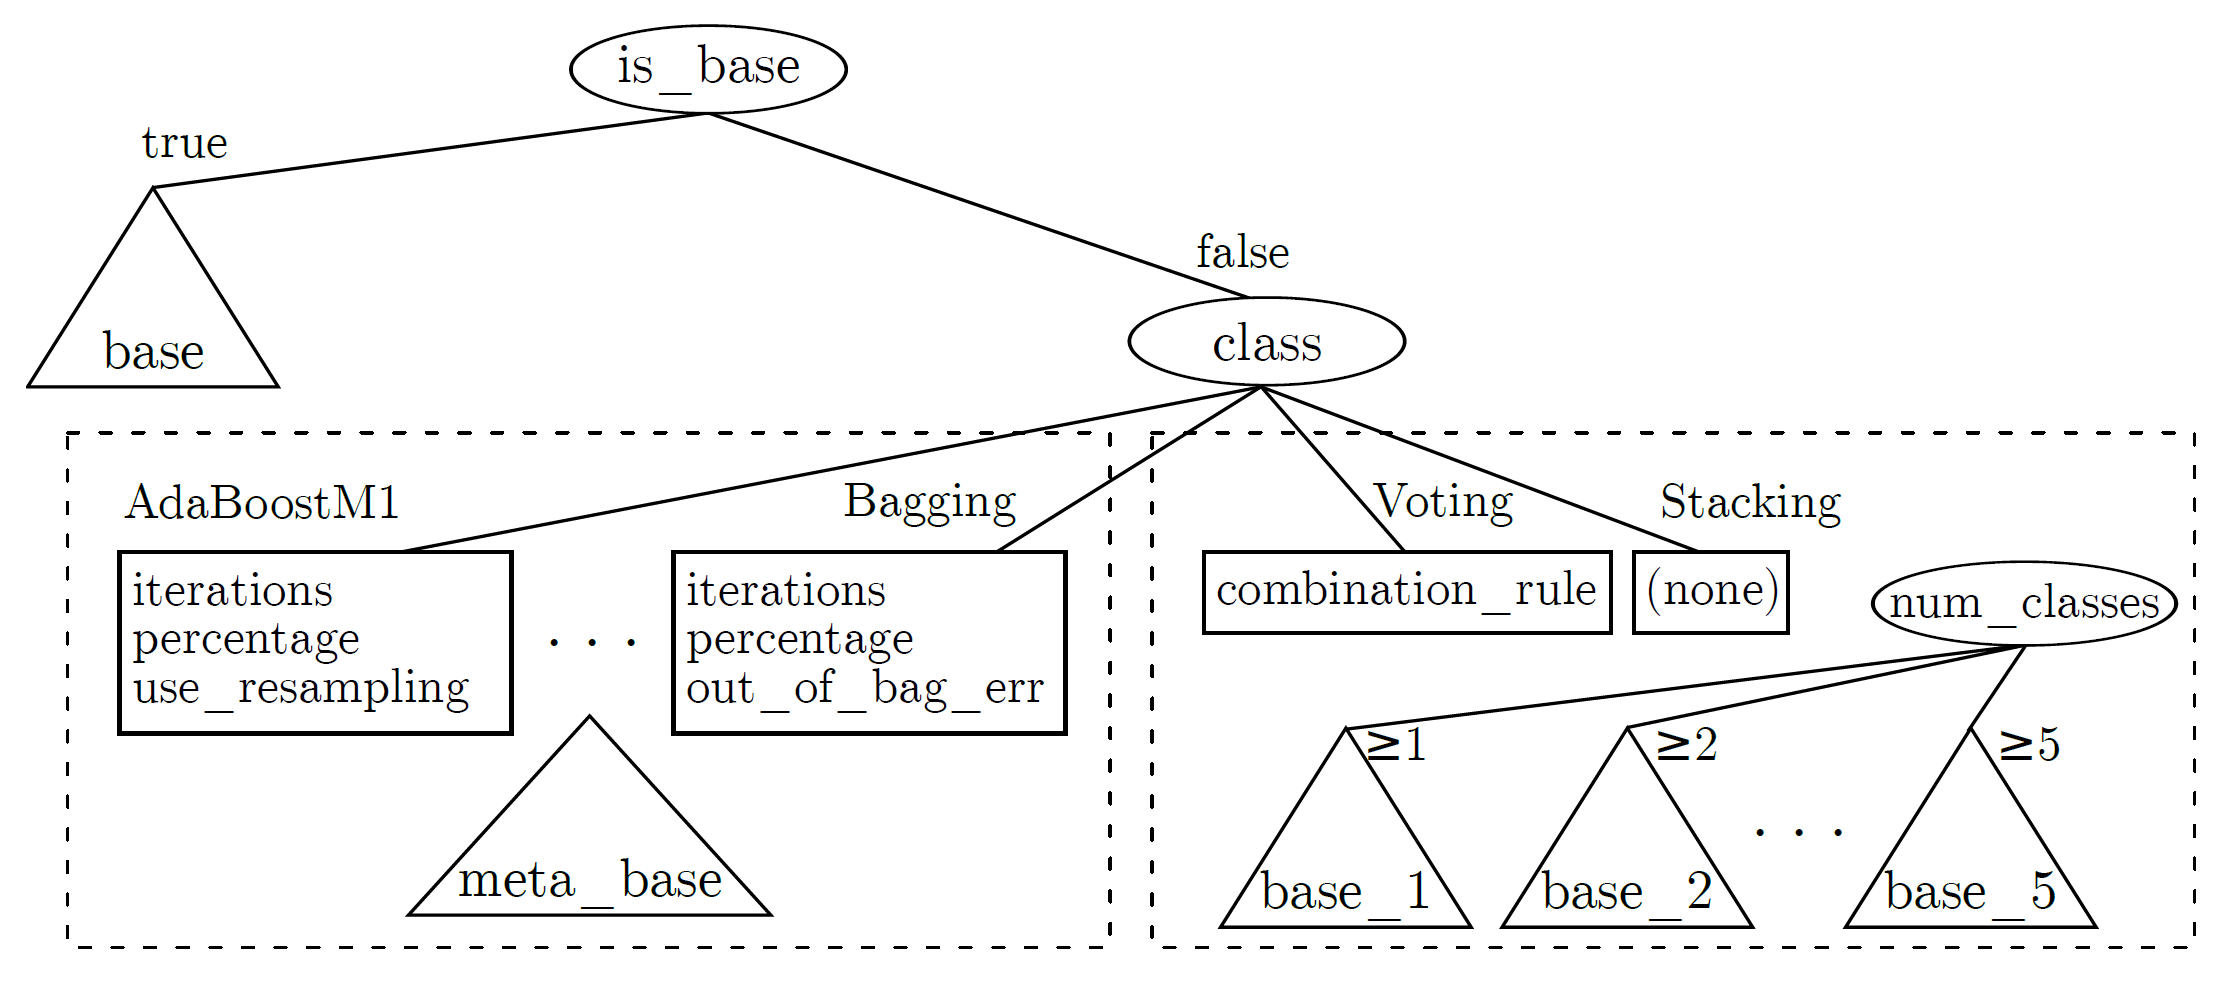
\includegraphics[width=\linewidth, keepaspectratio=true]{images/success_stories/AutoWEKA_space.png}
    }
\end{columns}

\onslide<4->
    \myit{
    \vspace*{-0.9cm}
    \item Results: 
        \myit{
                \item \alert{Better than an oracle of the 26 base classifiers} with default hyperparameters
                \item \alert{100$\times$ faster than grid search} over base classifiers, and still better in 14/21 cases
                \item Better than the only other applicable method TPE in \alert{19/21 cases}
        }
    \item Impact for practitioners: Auto-WEKA plugin was downloaded tens of thousands of times
    }

\end{frame}

%-----------------------------------------------------------------------

%-----------------------------------------------------------------------
\begin{frame}[c]{Questions to Answer for Yourself / Discuss with Friends}

\begin{itemize}
    \item \alert{Repetition.} List several success stories of Bayesian optimization
\medskip
    \item \alert{Repetition.} List several prominent tools for Bayesian optimization
\medskip
    \item \alert{Discussion.} Recall the algorithm selection  problem; how does CASH relate to this (after all, it also has ``algorithm selection'' as part of its name)? 
    (Hint: they are quite different.)
\end{itemize}

\end{frame}